\section{Parallelisierungsschema}

%----------------------------------------------------------------------%SLIDE -
\begin{frame}
    \frametitle{Parallelisierungsschema}

    Was ist parallelisierbar?
    \begin{itemize}
        \con
            Die Generationen sind inherent sequentiell
        \pro
            die einzelnen Spiele sind unabhängig voneinander
            (\textbf{for} $net_a, net_b \in N_i$ \textbf{do})
        \unknown
            die Ausgabeberechnung in den Neuronalen Netzwerken
            (dreifache Schleife)
    \end{itemize}
\end{frame}
%----------------------------------------------------------------------%SLIDE -

%----------------------------------------------------------------------%SLIDE -
\begin{frame}
    \frametitle{Parallelisierung der Spielphase}

    \begin{columns}[t]
        \column{0.5\textwidth}
        \vspace{-0.7cm}
        \begin{algorithm}[H]
            \caption{parallele Spielphase (1)}
            \begin{algorithmic}[1]
                \For {Generation $i = 0$ bis $\ldots$}
                    \ParDo {$\forall net_a \in N_i$}
                        \ParDo {$\forall net_b \neq net_a \in N_i$}
                            \State lass $net_a, net_b$ spielen
                            \State zähle die Siege ($wins$)
                        \EndParDo
                    \EndParDo
                    \State \Call{reduce}{$wins$}
                    \IIf {rank = 0}
                        generiere $N_{i+1}$
                    \EndIIf
                    \State \Call{broadcast}{$N_i$, 0}
                \EndFor
            \end{algorithmic}
        \end{algorithm}
        \hfill

        \column{0.5\textwidth}
        Ziel: $n^2$ Spiele auf $p$ Prozesse zu verteilen
        \begin{itemize}
            \item Master erstellt $N_{i+1}$.
            \item Master sendet $N_{i+1}$ an alle.
            \item Gleichmäßige Verteilung der inneren Schleifen (Zeilen 3,4).
        \end{itemize}
        Probleme:
        \begin{itemize}
            \item $\approx \SI{100}{\kibi\byte}$ pro Netzwerk
            \item viele kollektive Operationen
        \end{itemize}
    \end{columns}
\end{frame}
%----------------------------------------------------------------------%SLIDE -

%----------------------------------------------------------------------%SLIDE -
\begin{frame}
    \frametitle{Parallelisierung der Spielphase}

    \begin{columns}[t]
        \column{0.5\textwidth}
        \vspace{-0.7cm}
        \begin{algorithm}[H]
            \caption{parallele Spielphase (2)}
            \begin{algorithmic}[1]
                \For {Generation $i = 0$ bis $\ldots$}
                    \ParDo {$\forall net_a \in N_i$}
                        \ParDo {$\forall net_b \neq net_a \in N_i$}
                            \State lass $net_a, net_b$ spielen
                            \State zähle die Siege ($wins$)
                        \EndParDo
                    \EndParDo
                    \State \Call{reduce}{$wins$}
                    \State generiere $N_{i+1}$
                \EndFor
            \end{algorithmic}
        \end{algorithm}
        \hfill

        \column{0.5\textwidth}
        Ziel: $n^2$ Spiele auf $p$ Prozesse zu verteilen
        \begin{itemize}
            \item \emph{Jeder} erstellt $N_{i+1}$.
            \item \sout{Master sendet $N_{i+1}$ an alle.}
            \item Gleichmäßige Verteilung der inneren Schleifen (Zeilen 3,4).
        \end{itemize}
        Probleme:
        \begin{itemize}
            \item \sout{$\approx \SI{27}{\kibi\byte}$ pro Netzwerk}
            \item \sout{viele kollektive Operationen}
            \item ?
        \end{itemize}
    \end{columns}
\end{frame}
%----------------------------------------------------------------------%SLIDE -

%----------------------------------------------------------------------%SLIDE -
\begin{frame}
    \frametitle{Not So Strong Scaling}

    \begin{figure}
        \centering
        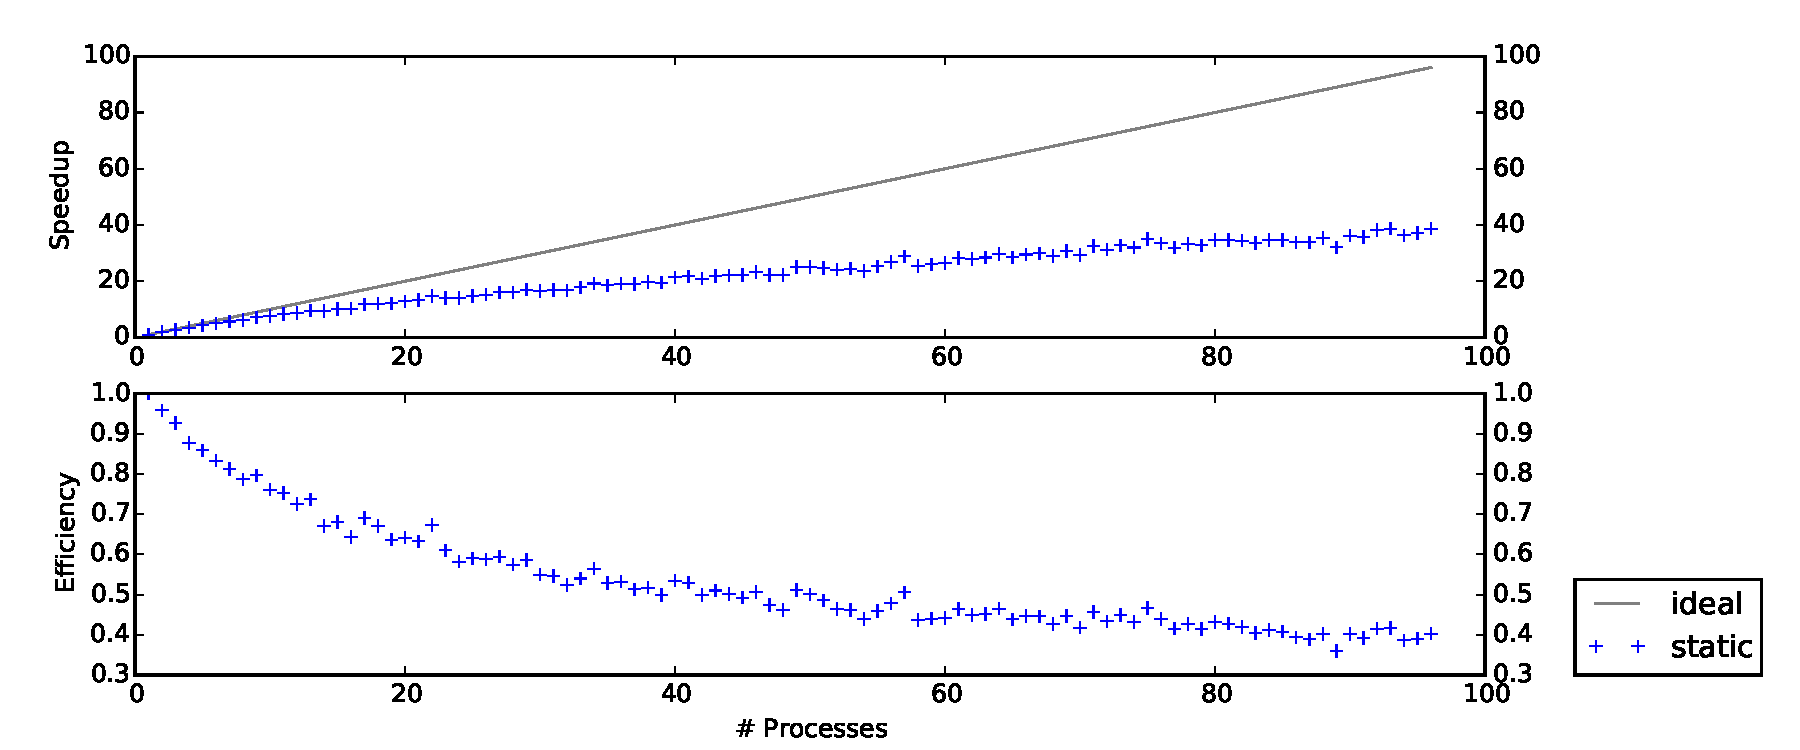
\includegraphics[width=\textwidth]{content/img/strong_scaling_time_static}
        %\caption{}
    \end{figure}

\end{frame}
%----------------------------------------------------------------------%SLIDE -

%----------------------------------------------------------------------%SLIDE -
\begin{frame}
    \frametitle{Not So Strong Scaling}
    \framesubtitle{Spurdatenanalyse}

    \begin{figure}
        \centering
        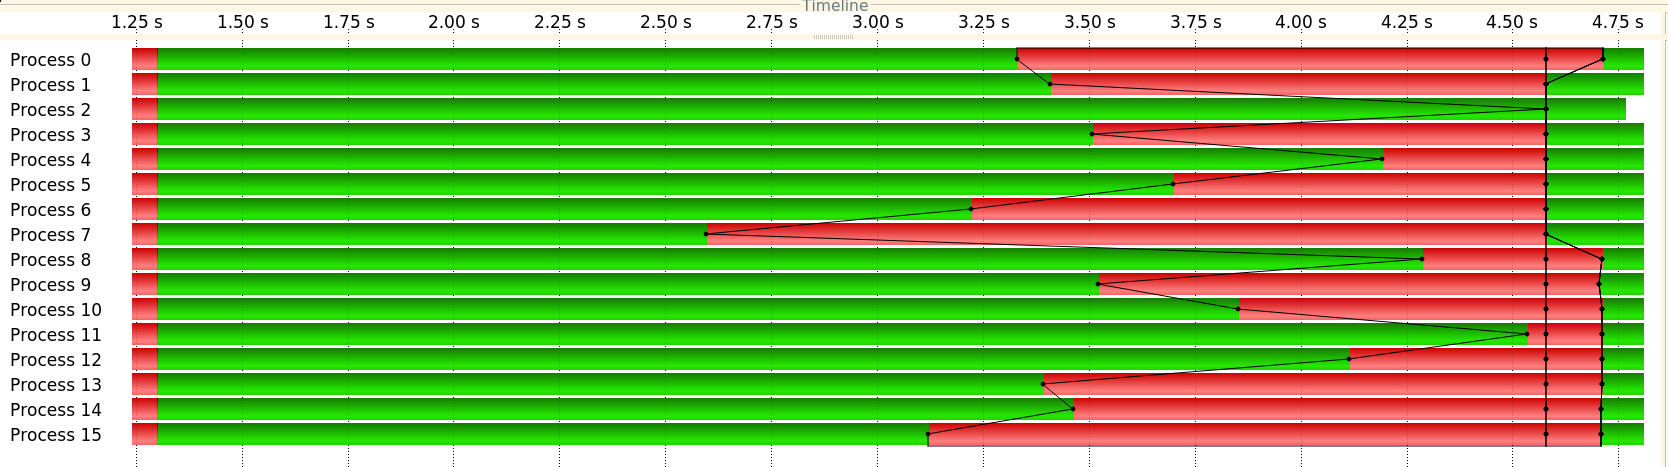
\includegraphics[width=\textwidth]{content/img/vampir_static}
        \caption{Vampir}
    \end{figure}

\end{frame}
%----------------------------------------------------------------------%SLIDE -

%----------------------------------------------------------------------%SLIDE -
\begin{frame}
    \frametitle{Not So Strong Scaling}

    Was ist da los?
    \begin{itemize}
        \item Spiele dauern unterschiedlich lange (2-1024 Züge)
        \item Länge ist nicht vorhersagbar
        \item[$\Rightarrow$] Lastungleichheit zwischen den Prozessen
    \end{itemize}

    %\pause
    \hfill

    Lösung: Dynamisches Scheduling
    \begin{itemize}
        \item Master/Worker Modell
        \item ein Anteil der Spiele wird gleichmäßig verteilt ($initial$)
        \item Master verteilt restliche Spiele paketweise an idlende Prozesse
              ($chunksize$)
    \end{itemize}

\end{frame}
%----------------------------------------------------------------------%SLIDE -

%----------------------------------------------------------------------%SLIDE -
\begin{frame}
    \frametitle{Dynamic Scheduling}

    \begin{columns}[t]
        \column{0.5\textwidth}
        \vspace{-0.7cm}
        \begin{algorithm}[H]
            \caption{Master}
            \begin{algorithmic}[1]
                \Require $initial, chunksize, n$ (number of games)
                \State $start \gets n \cdot initial$
                \While {$start < n$}
                    \State $msg, p \gets $\Call{Recv}{?}
                    \State \Call{Send}{$p, (start, chunksize)$}
                    \State $start \gets start + chunksize$
                \EndWhile
                \For {each process $p$}
                    \State $msg, p \gets $\Call{Recv}{?}
                    \State \Call{Send}{$p, (0, 0,$ "nothing to do")}
                \EndFor
            \end{algorithmic}
        \end{algorithm}

        \column{0.5\textwidth}
        \vspace{-0.7cm}
        \begin{algorithm}[H]
            \caption{Worker}
            \begin{algorithmic}[1]
                \Require initial, chunksize, number of games
                \State $start, chunksize \gets \Call{partition}{n \cdot initial}$
                \While {$chunksize \neq 0$}
                    \For {$g \in [start, start + chunksize)$}
                        \State rechne Game $\#g$
                        \State zähle die Siege ($wins$)
                    \EndFor
                    \State \Call{Send}{$master$, "{}I'm bored"}
                    \State $start, chunksize \gets $\Call{Recv}{$master$}
                \EndWhile
            \end{algorithmic}
        \end{algorithm}
    \end{columns}
\end{frame}
%----------------------------------------------------------------------%SLIDE -

%----------------------------------------------------------------------%SLIDE -
\begin{frame}
    \frametitle{Stronger Scaling}
    \framesubtitle{Chunksize}

    \begin{figure}
        \centering
        \centering
        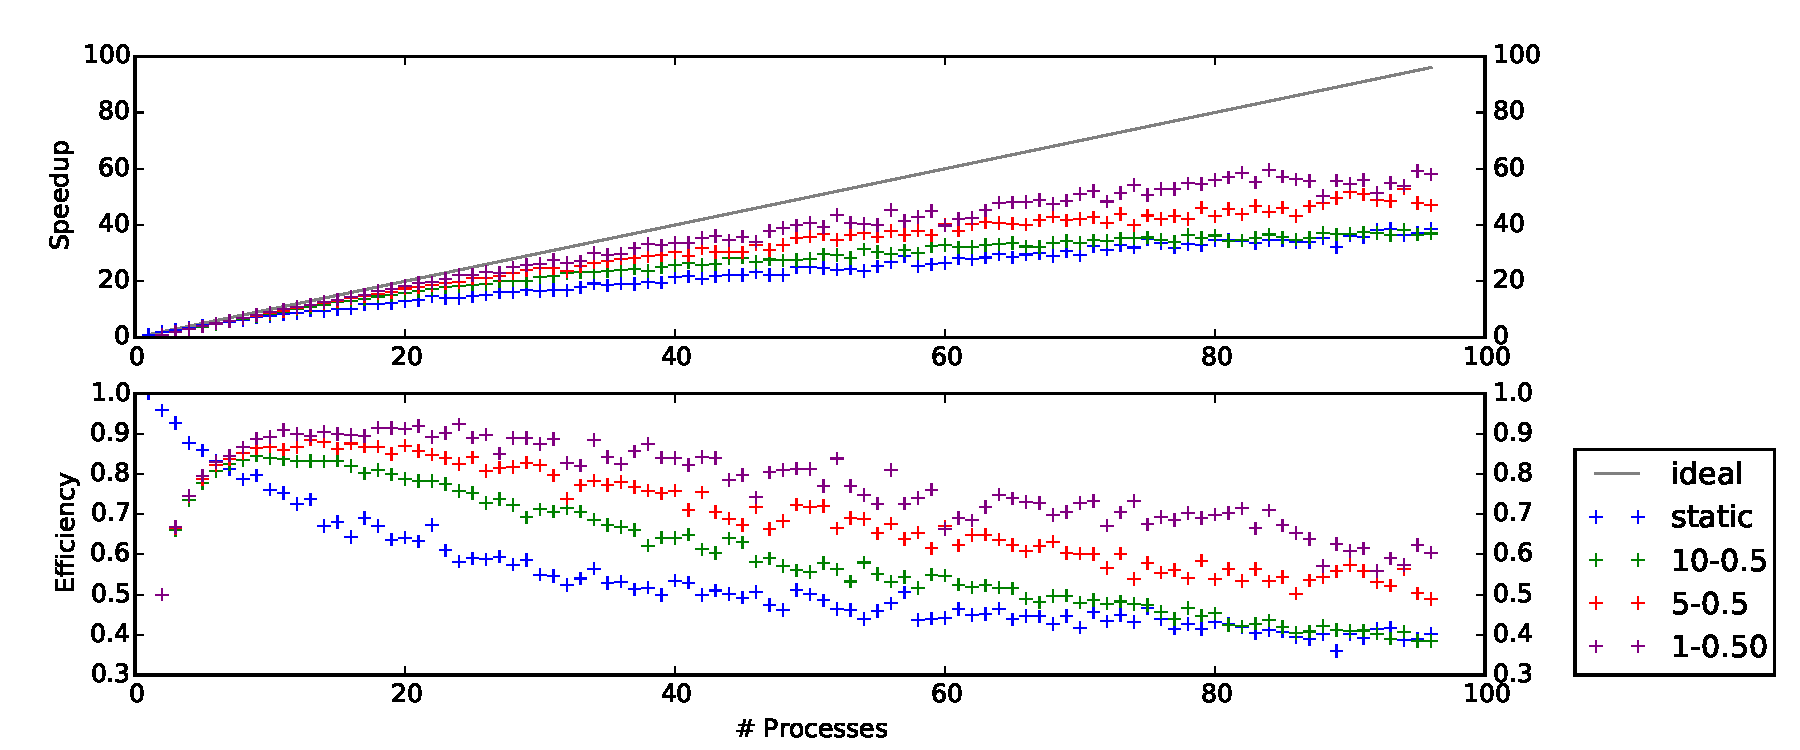
\includegraphics[width=\textwidth]{content/img/strong_scaling_time_chunksize}
        %\caption{}
    \end{figure}

\end{frame}
%----------------------------------------------------------------------%SLIDE -

%----------------------------------------------------------------------%SLIDE -
\begin{frame}
    \frametitle{Stronger Scaling}
    \framesubtitle{Initial}

    \begin{figure}
        \centering
        \centering
        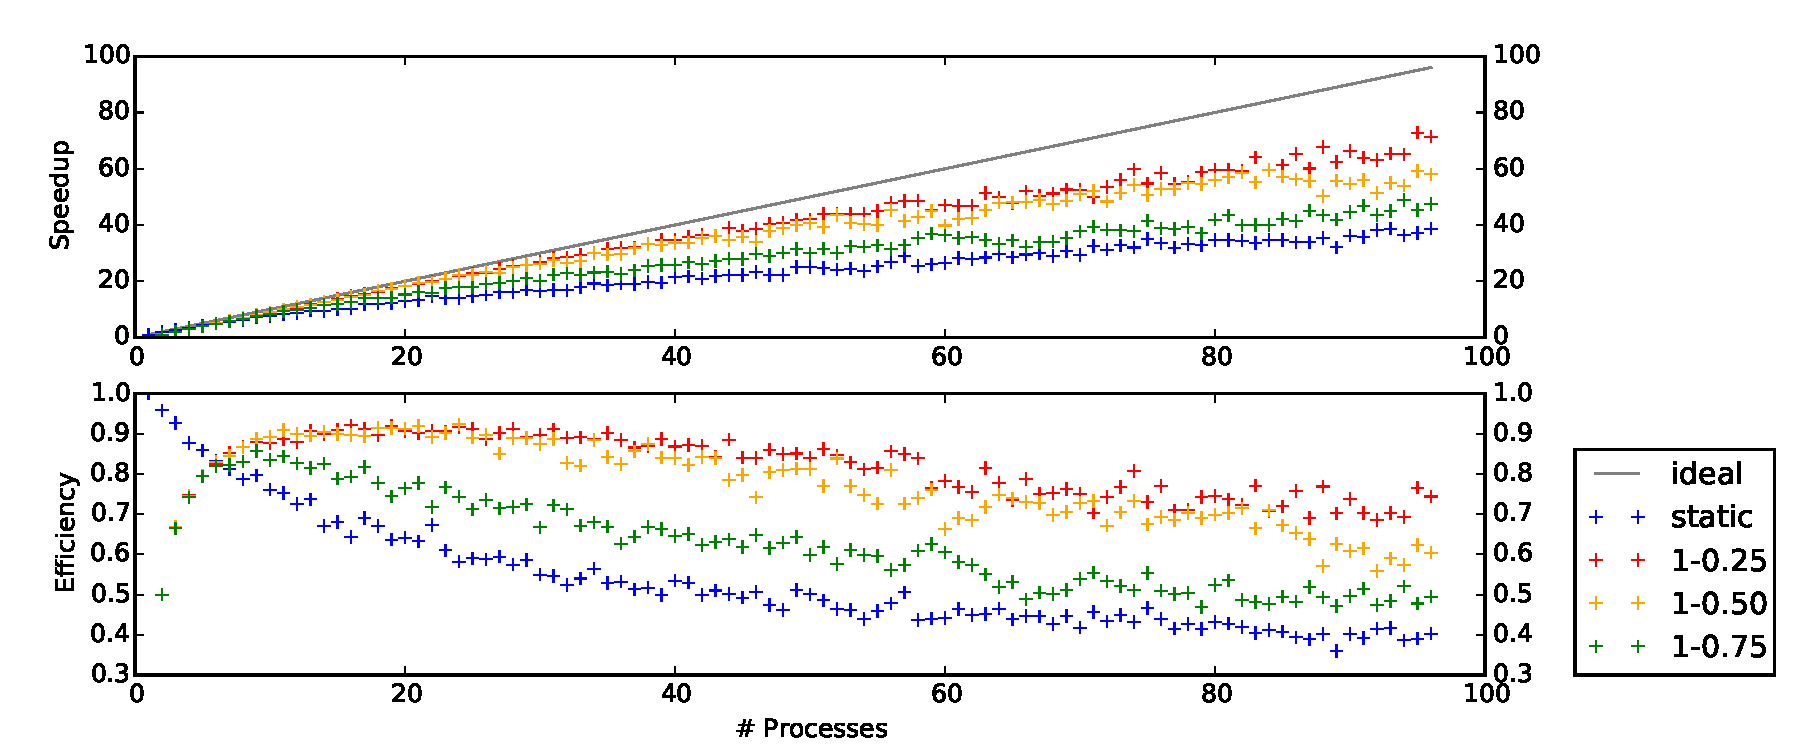
\includegraphics[width=\textwidth]{content/img/strong_scaling_time_initial}
        %\caption{}
    \end{figure}

\end{frame}
%----------------------------------------------------------------------%SLIDE -

%----------------------------------------------------------------------%SLIDE -
\begin{frame}
    \frametitle{Much Stronger Scaling}
    \framesubtitle{{}}

    \begin{figure}
        \centering
        \centering
        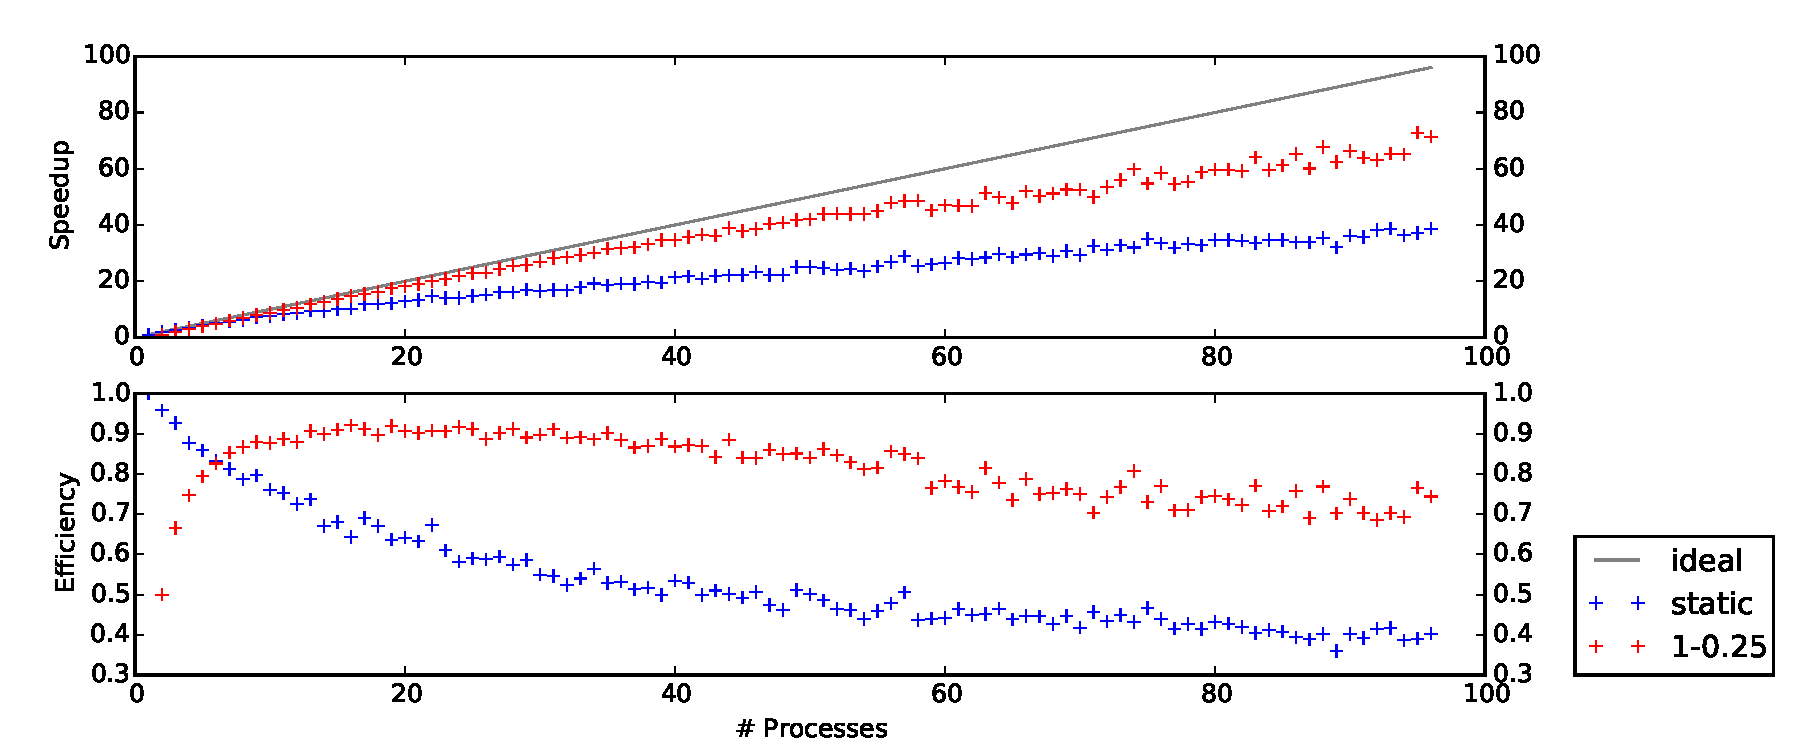
\includegraphics[width=\textwidth]{content/img/strong_scaling_time_final}
        %\caption{}
    \end{figure}

\end{frame}
%----------------------------------------------------------------------%SLIDE -

%----------------------------------------------------------------------%SLIDE -
\begin{frame}
    \frametitle{Much Stronger Scaling}
    \framesubtitle{Spurdatenanalyse}

    \begin{figure}
        \centering
        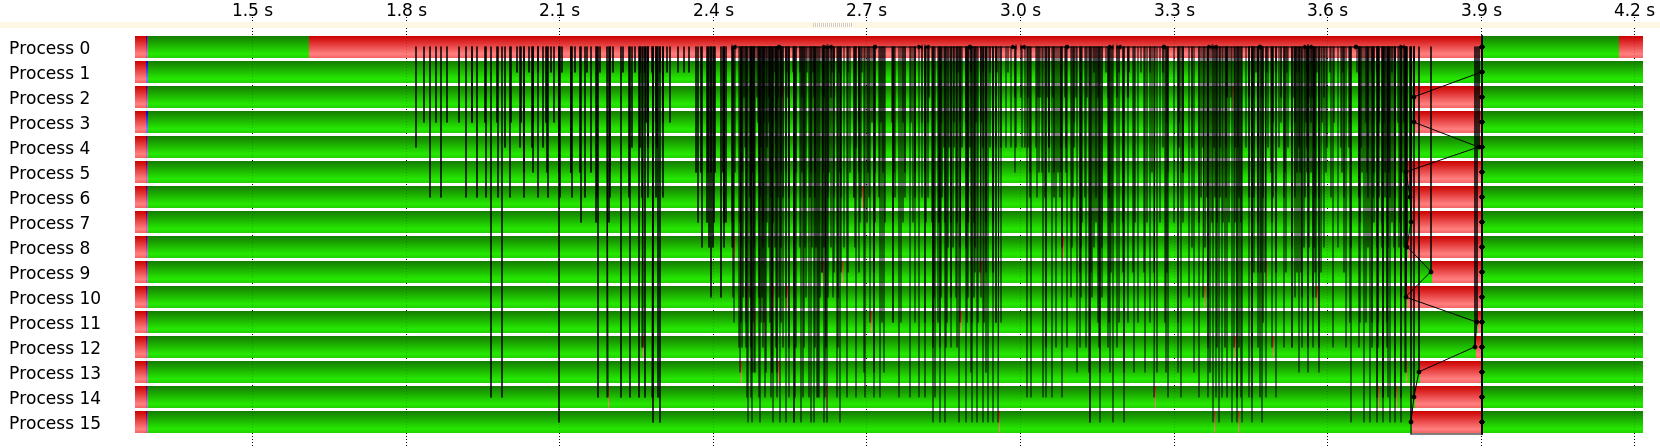
\includegraphics[width=\textwidth]{content/img/vampir_dynamic}
        \caption{Vampir}
    \end{figure}

\end{frame}
%----------------------------------------------------------------------%SLIDE -

%----------------------------------------------------------------------%SLIDE -
\begin{frame}
    \frametitle{Parallelisierung der neuronalen Netzwerke (OpenMP)}
    \begin{columns}[t]
        \column{0.6\textwidth}
        \vspace{-0.5cm}
        \begin{algorithm}[H]
            \caption{output calculation}
            \begin{algorithmic}[1]
                \Require in
                \Ensure out
                \For {each $gap$}
                    \State \Call{init}{out}
                    \ParDo {$from \gets 0$ to $neurons\_per\_layer[gap]$}
                        \For {$to \gets 0$ to $neurons\_per\_layer[gap+1]$}
                        \State $out[to] \gets out[to] +{}$
                        \State $\qquad\qquad\;\; in[from] * edges[gap][from][to]$
                        \EndFor
                    \EndParDo
                    \State \Call{swap}{in, out}
                \EndFor
            \end{algorithmic}
        \end{algorithm}
        \column{0.4\textwidth}
        \vspace{-0.5cm}
        \begin{itemize}
            \item Ist langsam.
            \item Je mehr Prozesse desto langsamer.
            \item Vermutlich zu hoher Overhead durch Fork/Join bei wenig Iterationen.
        \end{itemize}
    \end{columns}
\end{frame}
%----------------------------------------------------------------------%SLIDE -
